\documentclass[11pt]{article}
\usepackage[utf8]{inputenc}
\usepackage[T1]{fontenc}
\usepackage[spanish,es-noshorthands,es-tabla]{babel}
\usepackage{mathptmx}
\usepackage[margin=2.5cm]{geometry}
\usepackage{graphicx,subcaption,booktabs,float,setspace,caption}
\usepackage[hidelinks]{hyperref}
\graphicspath{{../figuras/}}
\captionsetup{font=small,labelfont=bf}
\setstretch{1.15}
\newcommand{\nota}[1]{\begin{minipage}{0.95\linewidth}\footnotesize #1\end{minipage}}

\title{¿Explica la cerveza la anemia infantil en Puno?}
\author{Carlos Chávez}
\date{Noviembre de 2026}

\begin{document}
\maketitle

\begin{abstract}
\noindent Puno está entre los departamentos donde más cerveza se adquiere por persona, y también fue durante años el departamento con mayor anemia infantil. Con microdatos de la ENDES, la ENAHO y la ENAPREF encuentro que el consumo de alcohol que miden las encuestas explica casi nada de la brecha de anemia entre Puno y el resto del país. Aun si todos los adultos dejaran de beber, la anemia en Puno bajaría alrededor de un punto porcentual. La brecha depende sobre todo de cómo se corrige la hemoglobina por altitud. Con el criterio de la OMS de 2024 la diferencia pasa de 31 a 8 puntos y Puno deja de ser el departamento con más anemia. El alcohol sí aparece asociado con otros daños. Cuando la pareja se embriaga con frecuencia, la violencia física o sexual contra la mujer es 23 puntos mayor.
\end{abstract}

\section{La pregunta}

Hace poco circuló en redes la idea de que la anemia infantil de Puno se explica porque las familias gastan en cerveza lo que deberían gastar en alimentar a sus hijos. La idea es atractiva porque junta dos hechos conocidos. Puno tiene una de las tasas de anemia infantil más altas del Perú y tiene fama de consumir mucha cerveza, sobre todo en sus fiestas. Si el gasto en alcohol desplazara alimentos ricos en hierro, la relación sería directa. Pero que dos cosas ocurran en el mismo lugar no significa que una cause la otra, y por eso quise ver qué dicen los datos.

Uso tres encuestas del INEI que miden el alcohol de manera distinta. La ENDES pregunta a un adulto de cada hogar si bebió, cuántas veces y cuánto en la ocasión de mayor consumo del mes, y además mide la hemoglobina de los niños. La ENAHO registra cuánto gasta el hogar en bebidas alcohólicas para consumir en casa. La ENAPREF de 2019 y 2020 registra en diarios de siete días todo lo que compra el hogar y cada uno de sus miembros, incluida la cerveza en bares y fiestas, y por eso es la mejor fuente para medir litros. Ninguna de las tres permite estimar efectos causales, de modo que todo lo que sigue son asociaciones condicionadas en características observables. La Figura~\ref{fig:mapas} resume el punto de partida.

\begin{figure}[!t]
\centering
\begin{subfigure}{0.30\linewidth}\centering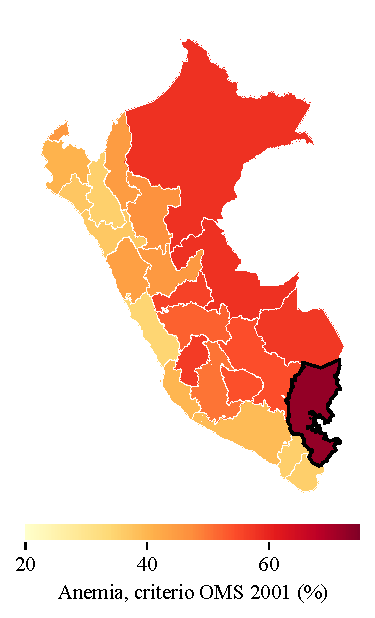
\includegraphics[width=\linewidth]{mapa_anemia_2001}\caption{Anemia, criterio OMS 2001}\end{subfigure}\hspace{1em}
\begin{subfigure}{0.30\linewidth}\centering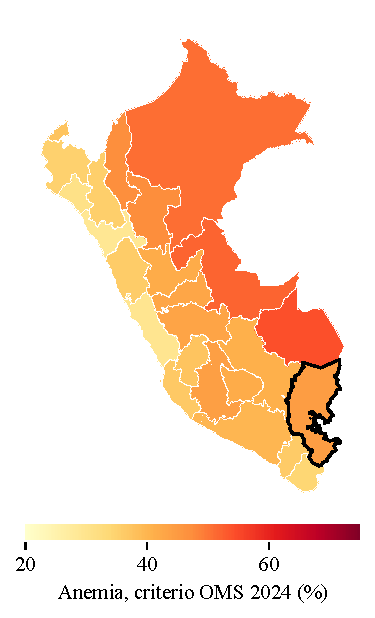
\includegraphics[width=\linewidth]{mapa_anemia_2024}\caption{Anemia, criterio OMS 2024}\end{subfigure}\\[0.6em]
\begin{subfigure}{0.30\linewidth}\centering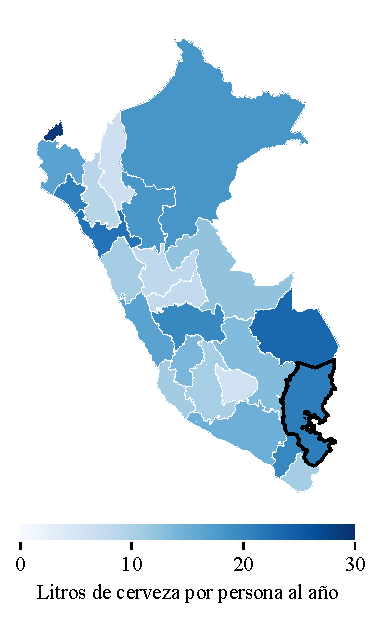
\includegraphics[width=\linewidth]{mapa_cerveza_enapref}\caption{Cerveza adquirida por persona}\end{subfigure}
\caption{Anemia infantil y cerveza por departamento}\label{fig:mapas}
\nota{Los paneles (a) y (b) muestran el porcentaje de niños de 6 a 35 meses con anemia en la ENDES 2014 a 2024, calculado con la hemoglobina medida y cada criterio de la OMS aplicado a todos los años. El panel (c) muestra los litros de cerveza adquiridos por persona al año según los diarios de gasto del hogar y personales de la ENAPREF 2019 a 2020. La ENAPREF es representativa de las ciudades y no de todo el departamento. Puno aparece con borde negro.}
\end{figure}

\section{¿Se toma más en Puno?}

La respuesta depende de qué se mida, y la Figura~\ref{fig:indice} lo muestra con seis indicadores de tres encuestas. La fila de arriba mide cuánta gente bebe y con qué frecuencia. En la ENDES, el 27 por ciento de los adultos entrevistados en Puno bebió en el último mes, frente al 37 por ciento en el resto del país, y quienes bebieron lo hicieron 1,4 veces en promedio, frente a 1,9. Las mujeres de Puno, en cambio, describen otra cosa de sus parejas. El 83 por ciento dice que su pareja se embriaga a veces o con frecuencia, frente al 60 por ciento en el resto del país.

\begin{figure}[!t]
\centering
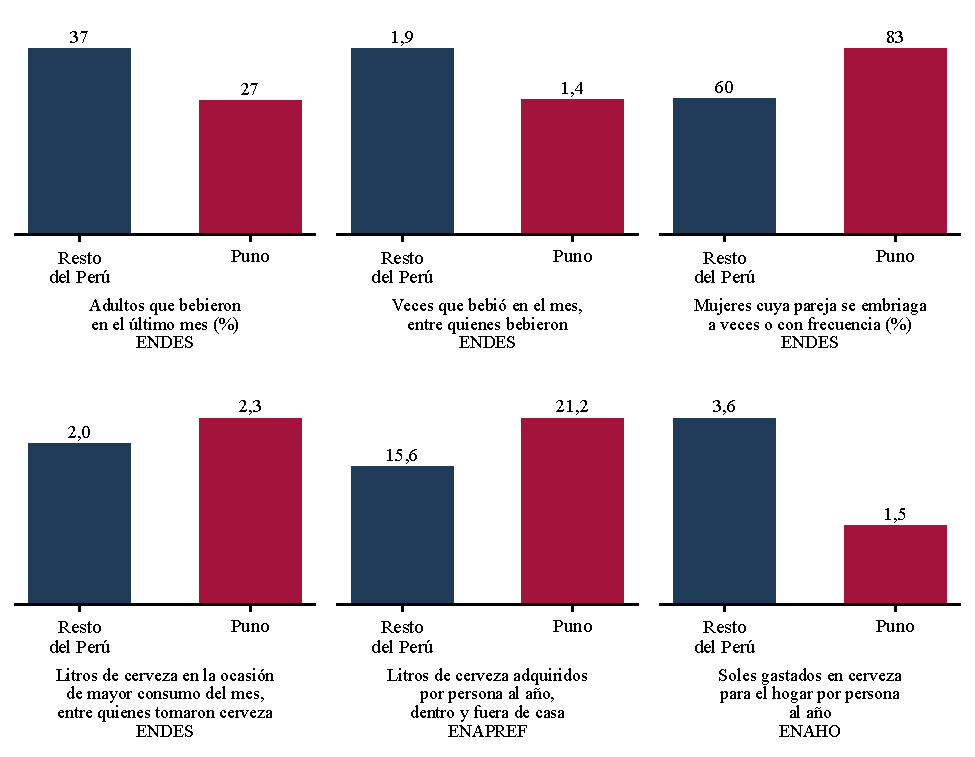
\includegraphics[width=0.80\linewidth]{puno_vs_resto_alcohol}
\caption{Consumo de alcohol en Puno y en el resto del Perú}\label{fig:indice}
\nota{Los paneles de arriba miden cuánta gente bebe y con qué frecuencia, y los de abajo cuánto se bebe o se compra. ENDES 2014 a 2024 para el adulto entrevistado en hogares con niños de 6 a 35 meses, ENDES 2010 a 2022 para las mujeres con pareja, ENAPREF 2019 a 2020 y ENAHO 2014 a 2024. En la ENDES la cantidad se pregunta para la ocasión en que más bebió el entrevistado en el último mes, contando 0,25 litros por vaso o lata y 0,62 litros por botella. El gasto de la ENAHO solo incluye la cerveza comprada para consumir en el hogar.}
\end{figure}

La fila de abajo mide cantidades y cuenta una historia distinta. Cuando los adultos de Puno toman cerveza, toman más. En su ocasión de mayor consumo del mes fueron 2,3 litros, frente a 2,0 en el resto del país. La ENAPREF, que registra en diarios todo lo que compran el hogar y cada uno de sus miembros, incluida la cerveza de bares y fiestas, muestra que en Puno se adquieren 21,2 litros de cerveza por persona al año, frente a 15,6 en el resto del país. El departamento ocupa el cuarto lugar de veinticinco con cualquiera de los cuatro métodos que usé para convertir las compras a litros, y en la zona urbana la diferencia es mayor, con 24,2 litros frente a 17,1. Esto coincide con la ENAPREF de 2008 y 2009, en la que la ciudad de Puno ocupaba el tercer lugar después de Iquitos y Moyobamba. La ENAHO, que solo registra la cerveza comprada para el hogar, apenas capta este consumo, y por eso en ella Puno aparece gastando menos.

Las cifras se reconcilian si en Puno bebe menos gente y con menos frecuencia, pero en cantidades grandes cuando bebe, como ocurre con la cerveza de las fiestas, que se compra en cajas y se toma fuera de la casa. Lo que no puedo confirmar con datos públicos es que Puno sea el departamento que más cerveza consume. Las ventas por departamento de las cerveceras no se publican, y en la ENAPREF Tumbes, Madre de Dios y La Libertad están por encima de Puno. Lo que sí puedo afirmar es que Puno está entre los departamentos de mayor adquisición de cerveza, de modo que la premisa del argumento tiene fundamento.

\section{La medición de la anemia}

Antes de preguntar cuánto explica el alcohol hay que mirar cómo se mide la anemia, porque en Puno eso cambia casi todo. La anemia se define comparando la hemoglobina con un umbral. Como en la altura la hemoglobina es naturalmente más alta, primero se le resta una corrección por altitud. En 2024 la OMS cambió esa corrección y bajó el umbral para los menores de dos años, y el Perú adoptó la nueva regla ese mismo año. A unos 3.800 metros la corrección antigua restaba alrededor de 3,1 gramos por decilitro y la nueva resta cerca de 2,6. Reconstruí ambas definiciones con la hemoglobina medida para todos los años desde 2010. Mis prevalencias nacionales difieren en 0,5 puntos o menos de las que publican Campos-Sánchez et al. (2025) con los mismos datos.

Con el criterio de 2001, la anemia en Puno en 2014 a 2024 fue de 72,8 por ciento, 30,9 puntos por encima del resto del país. Con el criterio de 2024 fue de 44,5 por ciento y la brecha baja a 8,0 puntos. Puno deja de ser el departamento con más anemia y queda detrás de Madre de Dios, Ucayali, Loreto, San Martín y Amazonas. La Figura~\ref{fig:criterio} separa los dos cambios de la regla. Si solo se cambia el umbral por edad, la brecha casi no se mueve. Si solo se cambia la corrección por altitud, cae a 6,8 puntos. Una descomposición de Shapley atribuye $-24{,}5$ puntos al ajuste por altitud y $+1{,}6$ al umbral por edad.

\begin{figure}[H]
\centering
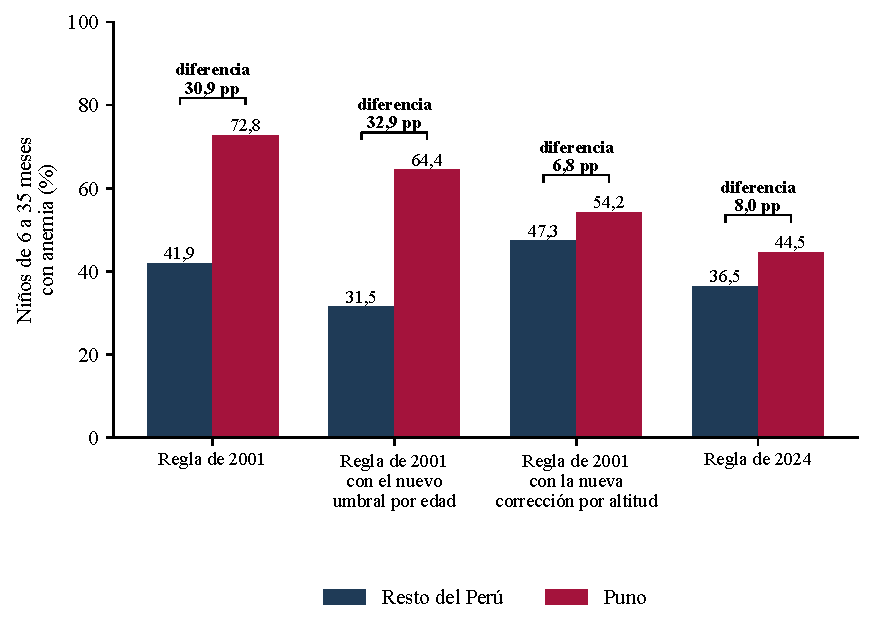
\includegraphics[width=0.72\linewidth]{brecha_por_criterio}
\caption{Brecha de anemia entre Puno y el resto del Perú según el criterio}\label{fig:criterio}
\nota{Diferencia en puntos porcentuales entre la anemia de niños de 6 a 35 meses en Puno y en el resto del Perú, ENDES 2014 a 2024. Las barras grises combinan un componente de cada regla para separar el efecto del ajuste por altitud y el del umbral por edad.}
\end{figure}

Esto no quiere decir que la anemia en Puno sea ficticia. La OMS cambió la corrección porque la anterior parecía exagerar la anemia en la altura, pero la evidencia sobre la magnitud correcta todavía es discutida. Lo que sí quiere decir es que cualquier explicación de la anemia de Puno tiene que pasar primero por la medición. Una parte grande de lo que se buscaba explicar con cerveza era el ajuste por altitud.

\section{¿Cuánto explica el alcohol?}

Para medir la relación entre alcohol y anemia estimo, a nivel de cada niño, modelos de probabilidad lineal con efectos fijos de departamento y año, y controles por edad y sexo del niño, quintil de riqueza, área, altitud, educación de la madre y edad y sexo del adulto entrevistado. Las asociaciones en el resto del país son positivas pero pequeñas, como muestra la Figura~\ref{fig:coef}. Cada litro adicional en la ocasión de mayor consumo se asocia con 0,4 puntos más de anemia, y que el adulto beba con frecuencia y reporte daños por el alcohol se asocia con 3,3 puntos más. En Puno los coeficientes son algo mayores, por ejemplo 4,2 puntos cuando el adulto tomó cerveza en su ocasión de mayor consumo, pero son imprecisos y ninguna diferencia con el resto del país es estadísticamente significativa.

\begin{figure}[H]
\centering
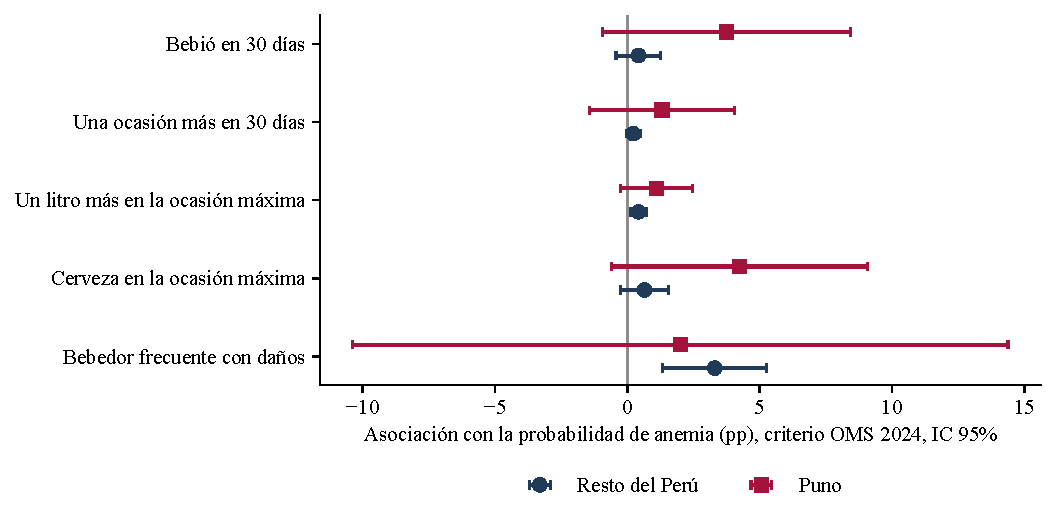
\includegraphics[width=0.72\linewidth]{coeficientes_anemia}
\caption{Asociación entre el consumo de alcohol del adulto y la anemia infantil}\label{fig:coef}
\nota{Coeficientes de modelos de probabilidad lineal estimados por separado para cada medida, con interacción con Puno. ENDES 2014 a 2024, anemia con criterio OMS 2024, errores estándar agrupados por conglomerado. Los resultados con el criterio de 2001 y excluyendo 2024 son similares.}
\end{figure}

La Tabla~\ref{tab:oaxaca} pregunta cuánto de la brecha de Puno se debe a que su consumo medido es distinto del resto. La respuesta es prácticamente nada. Con los cuatro indicadores de consumo, la contribución del alcohol es de $-0{,}1$ puntos con cualquiera de los dos criterios, porque en la ENDES Puno no bebe más y porque las asociaciones son pequeñas. La riqueza explica 3,5 puntos con ambos criterios. La altitud explica 15,4 puntos con el criterio de 2001 y resta 4,7 con el de 2024, lo que vuelve a mostrar que su papel depende de la corrección.

\begin{table}[H]
\centering
\caption{Descomposición de la brecha de anemia entre Puno y el resto del Perú}\label{tab:oaxaca}
\begin{tabular}{lcc}
\toprule
 & Criterio OMS 2001 & Criterio OMS 2024 \\
\midrule
Brecha total (pp) & 31,3 & 8,1 \\
\addlinespace
Consumo de alcohol del adulto & $-0{,}1$ & $-0{,}1$ \\
Quintil de riqueza & 3,5 & 3,6 \\
Altitud & 15,4 & $-4{,}7$ \\
Educación de la madre, área, edad y sexo del niño & $-0{,}5$ & $-0{,}3$ \\
Parte no explicada & 13,0 & 9,5 \\
\bottomrule
\end{tabular}\\[0.4em]
\nota{Descomposición de Oaxaca-Blinder con coeficientes de una regresión agrupada que incluye un indicador de Puno. ENDES 2014 a 2024. El consumo de alcohol incluye haber bebido en los últimos 30 días, el número de ocasiones, los litros en la ocasión de mayor consumo y ser bebedor frecuente con daños. La brecha difiere ligeramente de la Figura~\ref{fig:criterio} porque la muestra exige información completa del adulto entrevistado.}
\end{table}

Queda el contrafactual que plantea el argumento original. ¿Cuánto bajaría la anemia si los adultos dejaran de beber? Para responderlo estimo una sola regresión con los cuatro márgenes de consumo y sus interacciones con Puno, y simulo que todos valen cero. Con los coeficientes propios de Puno, la anemia bajaría 1,1 puntos, desde 44,3 por ciento, con un intervalo de confianza que va de $-2{,}3$ a $+0{,}2$. Con los coeficientes del resto del Perú bajaría 0,2 puntos. La Figura~\ref{fig:cf} muestra las tres simulaciones. Una reducción de dos tercios del consumo de cerveza tendría un efecto proporcionalmente menor. Hay que leer estos números como un máximo, porque suponen que toda la asociación es causal.

\begin{figure}[H]
\centering
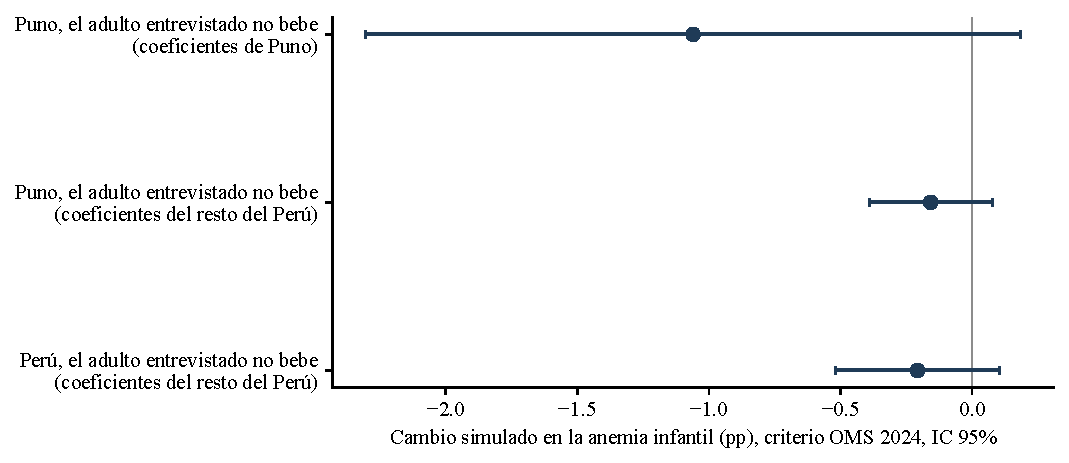
\includegraphics[width=0.68\linewidth]{contrafactual}
\caption{Cambio simulado en la anemia si el adulto entrevistado no bebiera}\label{fig:cf}
\nota{Cambio predicho en la anemia infantil al llevar a cero los cuatro indicadores de consumo del adulto, con intervalos de confianza al 95 por ciento por el método delta. ENDES 2014 a 2024, criterio OMS 2024.}
\end{figure}

El mecanismo del gasto tampoco aparece. En la ENAHO, los hogares con niños pequeños que compran cerveza, a igual gasto total, no destinan una proporción menor de su gasto en alimentos a carnes, hígado, sangrecita y pescado. La diferencia es de $-0{,}05$ puntos en todos los hogares y de $-0{,}4$ puntos en los hogares pobres, sin significancia estadística. El alcohol representa el 3,3 por ciento del gasto total de los hogares de Puno según la ENAPREF, frente al 2,3 por ciento en el país, y aun si todo ese dinero se dedicara a otros gastos la anemia cambiaría muy poco.

\section{Alcohol y bienestar de la familia}

Que el alcohol medido no explique la anemia de Puno no significa que el consumo excesivo no tenga costos. Donde la asociación es grande es en la violencia contra la mujer. En la ENDES de 2010 a 2022, comparadas con las mujeres cuya pareja no bebe, las mujeres cuya pareja se embriaga con frecuencia tienen 22,6 puntos más de probabilidad de haber sufrido violencia física o sexual en el último año, sobre un promedio de 11 por ciento, y 27,6 puntos más de violencia emocional. En Puno el aumento es casi el mismo, 23,6 puntos, como muestra la Figura~\ref{fig:violencia}. La diferencia está en la distribución. En Puno el 74 por ciento de las mujeres con pareja dice que esta se embriaga a veces, frente al 54 por ciento en el resto del país, y en esa categoría la violencia es 7,1 puntos mayor que entre las mujeres cuya pareja no bebe, frente a 4,1 puntos en el resto.

\begin{figure}[H]
\centering
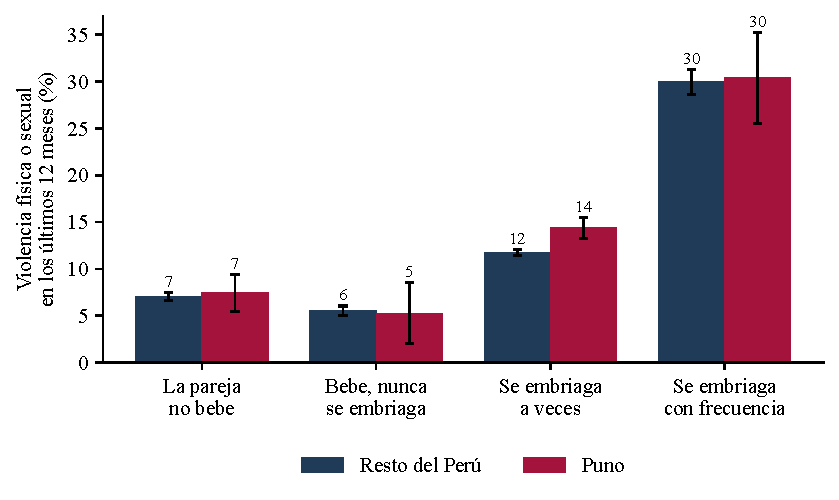
\includegraphics[width=0.72\linewidth]{violencia_por_consumo_pareja}
\caption{Violencia contra la mujer según el consumo de alcohol de la pareja}\label{fig:violencia}
\nota{Porcentaje de mujeres con pareja que sufrieron violencia física o sexual en los últimos 12 meses, con intervalos de confianza al 95 por ciento. ENDES 2010 a 2022. En 2023 la pregunta cambió de cuántas veces la pareja se embriaga a cuántas veces toma, y los resultados de 2023 y 2024 se presentan por separado en la Tabla~\ref{tab:bienestar}.}
\end{figure}

Las otras dos dimensiones que revisé muestran asociaciones más pequeñas, como resume la Tabla~\ref{tab:bienestar}. En los meses de clases, los niños de 6 a 16 años de hogares que compran alcohol tienen 1,1 puntos menos de matrícula y 1,3 puntos menos de asistencia, sobre promedios cercanos al 97 por ciento. Sin controlar por el mes de la entrevista esta diferencia parecía unas cinco veces mayor, porque en verano se compra más alcohol y todavía no se ha matriculado a los niños. Con el panel de la ENAHO tampoco encuentro un empobrecimiento posterior robusto. Cada punto del presupuesto dedicado al alcohol se asocia con un crecimiento del gasto total 0,7 por ciento menor al año siguiente, pero cuando mido el gasto sin alcohol la diferencia cae a 0,2 por ciento y deja de ser significativa. Buena parte de la primera cifra se debía a que el propio gasto en alcohol forma parte del gasto total.

\begin{table}[H]
\centering
\caption{Alcohol y otros resultados del hogar}\label{tab:bienestar}
\begin{tabular}{lccc}
\toprule
 & Resto del Perú & Puno & Media \\
\midrule
\multicolumn{4}{l}{\textit{Violencia física o sexual (ENDES 2010 a 2022, pp)}} \\
Pareja bebe pero nunca se embriaga & $-1{,}1$ (0,3) & $-1{,}7$ (1,8) & 11,0 \\
Pareja se embriaga a veces & 4,1 (0,3) & 7,1 (1,3) & \\
Pareja se embriaga con frecuencia & 22,6 (0,7) & 23,6 (2,6) & \\
\addlinespace
\multicolumn{4}{l}{\textit{Violencia física o sexual (ENDES 2023 a 2024, pregunta nueva, pp)}} \\
Pareja toma con mucha frecuencia & 18,6 (1,8) & 17,5 (8,3) & \\
\addlinespace
\multicolumn{4}{l}{\textit{Escolaridad de niños de 6 a 16 años (ENAHO, meses de clases, pp)}} \\
Matrícula, el hogar compra alcohol & \multicolumn{2}{c}{$-1{,}1$ (0,2)} & 96,9 \\
Asistencia, el hogar compra alcohol & \multicolumn{2}{c}{$-1{,}3$ (0,2)} & 96,2 \\
\addlinespace
\multicolumn{4}{l}{\textit{Bienestar al año siguiente (panel ENAHO, por punto de presupuesto en alcohol)}} \\
Crecimiento del gasto total (\%) & \multicolumn{2}{c}{$-0{,}69$ (0,12)} & \\
Crecimiento del gasto sin alcohol (\%) & \multicolumn{2}{c}{$-0{,}22$ (0,13)} & \\
Probabilidad de pobreza (pp) & \multicolumn{2}{c}{0,29 (0,13)} & \\
\bottomrule
\end{tabular}\\[0.4em]
\nota{Errores estándar agrupados entre paréntesis. En violencia se compara con las mujeres cuya pareja no bebe, con controles por edad, educación, quintil de riqueza, área, departamento y año. En escolaridad se usan efectos fijos de departamento, año y mes, y controles por gasto per cápita, tamaño del hogar, edad y sexo, de abril a noviembre. En bienestar se usan los paneles 2011 a 2015, 2015 a 2019 y 2019 a 2023 enlazados con el módulo de alimentos, con controles por gasto, pobreza y tamaño del hogar en el año inicial. La pobreza oficial se mide con un gasto que incluye el alcohol.}
\end{table}

\section{Conclusión}

Puno tiene buenas razones para su fama de consumir mucha cerveza. Los diarios de gasto de la ENAPREF lo ubican entre los cuatro departamentos con mayor adquisición por persona, y sus bebedores toman más por ocasión que los del resto del país, aunque beban con menos frecuencia. Pero eso no explica la anemia de sus niños. El consumo que miden las encuestas aporta casi nada a la brecha con el resto del país, los hogares que compran cerveza no gastan menos en alimentos ricos en hierro y, aun eliminando todo el consumo de los adultos, la anemia bajaría alrededor de un punto. La mayor parte de la brecha depende de cómo se corrige la hemoglobina por la altura, y con la regla actual de la OMS Puno ya no es el departamento con más anemia. Lo que el alcohol sí acompaña es la violencia contra las mujeres, que se cuadruplica cuando la pareja se embriaga con frecuencia. Si hay una razón para preocuparse por el consumo de cerveza en Puno, está más en los hogares donde se bebe hasta embriagarse que en la anemia de los niños.

\section*{Datos y métodos}

\small
Las regresiones de anemia usan 90.949 niños de 6 a 35 meses con hemoglobina medida en la ENDES de 2014 a 2024, sin 2020, cuyo hogar tiene un adulto entrevistado en el cuestionario de salud. La anemia se reconstruye con la hemoglobina medida (variable hc53), la altitud del conglomerado y las correcciones de la OMS. La corrección de 2001 es la ecuación del CDC, que se aplica cuando es positiva, y la de 2024 es la ecuación de la guía de la OMS. Los umbrales son 11,0 gramos por decilitro, o 10,5 para menores de 24 meses con el criterio de 2024. Las preguntas sobre cantidad de alcohol (QS212) se refieren a la ocasión de mayor consumo en los últimos 30 días y no a una ocasión típica, y las preguntas sobre daños (QS713 a QS717) solo se hacen a quienes beben 12 o más días al año. Los litros de la ENAPREF salen de la equivalencia declarada para el 54 por ciento del volumen, de la conversión por tamaño de envase para el 45 por ciento y de la imputación por precio para el 2 por ciento restante. El gasto en alcohol de la ENAHO corresponde a los productos con código 44 del módulo de alimentos. Una simulación alternativa, que trata el gasto en alcohol como ingreso adicional y usa el gradiente de anemia por riqueza, da una reducción de 0,4 puntos en Puno, pero depende de comparar quintiles de riqueza de la ENDES con quintiles de gasto de la ENAHO. Todos los cálculos se pueden reproducir con los programas del proyecto.

\section*{Referencias}

\small
\noindent Campos-Sánchez, M., L. Cordero-Muñoz, E. Velásquez-Hurtado, N. Baiocchi-Ureta, M. Miranda-Cuadros, M. I. Sánchez-Griñán y W. Valdivia-Miranda (2025). Nueva directriz de la Organización Mundial de la Salud sobre los puntos de corte de anemia. Implicancias en niños de 6 a 35 meses de Perú. \textit{Revista Peruana de Medicina Experimental y Salud Pública} 42(2), 115--125.

\noindent Instituto Nacional de Estadística e Informática. Encuesta Demográfica y de Salud Familiar 2010 a 2024, Encuesta Nacional de Hogares 2010 a 2024 y panel 2011 a 2023, y Encuesta Nacional de Presupuestos Familiares 2019 a 2020. Microdatos.

\noindent Organización Mundial de la Salud (2024). \textit{Guideline on haemoglobin cutoffs to define anaemia in individuals and populations}. Ginebra.

\end{document}
